\documentclass[12pt,a4paper]{article}
\usepackage[latin1]{inputenc}
\usepackage{amsmath}
\usepackage{amsfonts}
\usepackage{amssymb}
\usepackage{graphicx}
% \usepackage{url}
\usepackage{hyperref}
\usepackage{tikz}
\numberwithin{equation}{section}
% If you're editing this, please add your name to the authors list, and please do not take any names out. Adding to the list should be done like so,
% \author{Alice, Bob, Charlie, foo, etc.}
\author{Ian ``Comrade Pingu'' Mitchell\footnote{\url{Ian.Mitchell_001@gmx.com}}} 
\title{KSP Orbital Mechanics and Rocket Design}
\date{\today}

\graphicspath{ {/home/ian/Documents/'KSP Orbital Mechanics'/}}

\begin{document}

\maketitle

\begin{abstract}

	This document contains some essential formulas for designing rockets and preparing for adjusting orbits in Kerbal Space Program. This document was referenced from Scott Manley's \textit{Orbital Mechanics on Paper} series, and the \textit{Rocket Design Cheat Sheet} on the KSP Wiki. All of the formulas, equations, and diagrams are in near verbatim to each of these references. I do not intend to plagarize, but make an easy paper to reference when needed.
	
\end{abstract}

\section{The Essentials}

\begin{figure}[h]
	\centering
	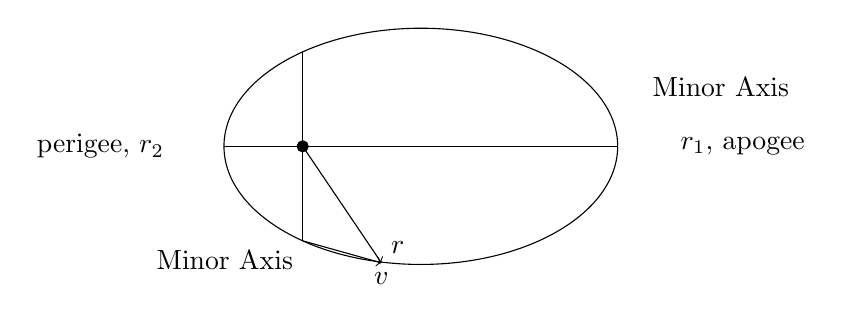
\begin{tikzpicture}
		% Lines and shapes
		\draw (2.5, 0) ellipse (2.5 and 1.5);
		\filldraw[black] (1,0) circle (2pt);	
		\draw (1, 0) -- (1, 1.2);
		\draw (1, 0) -- (1, -1.2) node[anchor=north east] {Minor Axis};
		\draw (0, 0) -- (5, 0);
		\draw[->] (1, -1.2) .. controls (1.5, -1.34) .. (2, -1.48) node[anchor=north] {$v$};
		% Text, math stuff, and distance
		\draw[->] (1, 0) -- (2, -1.48) node[anchor=south west] {$r$};
		\node[anchor=east] at (7.5, 0) {$r_1$, apogee};
		\node[anchor=west] at (-2.5, 0) {perigee, $r_2$};
		\node[anchor=north east] at (7.3, 1) {Minor Axis};
	\end{tikzpicture}
	\label{fig: 1}
	\caption{A particle is traveling at a velocity $v$ at a distance $r$ in an eccentric orbit near paregee.}
\end{figure}

\subsection{Semi-Major (average) Axis}

\begin{equation}
	a = \frac{r_1 + r_2}{2}
\end{equation}

In short, this is the relationship between the major and minor axis and the apogee and parigee. It simply bunches the average into one simple variable rather than having to have $(r_1 + r_2)/2$ in most every one of the equations in orbital mechanics.

\subsection{Velocity}

\begin{equation}
	v^2 = \mu \bigg{(}\frac{2}{r} - \frac{1}{a} \bigg{)}
\end{equation}
\begin{equation}
	v^2 = GM \bigg{(}\frac{2}{r} - \frac{1}{a} \bigg{)}
\end{equation}
\begin{equation}
	v = \sqrt{\mu \bigg{(}\frac{2}{r} - \frac{1}{a} \bigg{)}}
\end{equation}
where

\[ \mu = GM \]
\[ G = 6.67 \times 10^{-11} \text{ m$^{3}$ kg$^{-1}$ s$^{-2}$}\]

and $r$ is the distance from a planet's core, and $M$ is the mass of the body you're working with.\\\\

To summarize, the closer you get to a planet, the faster you move. The farther you are from a planet

\newpage

\section{Inclination Change}


\begin{figure}[h]
	\centering
	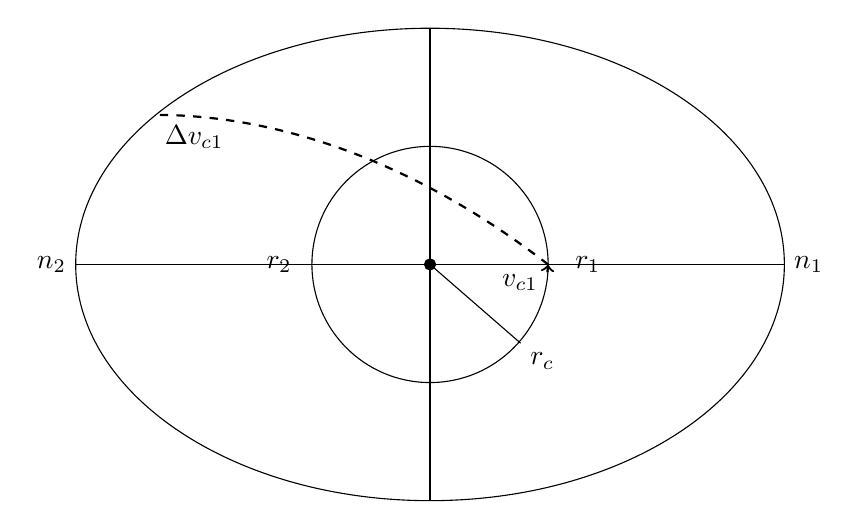
\begin{tikzpicture}
		% Grid for temporary reference

		% \draw[step=1.0cm,color=gray] (-5,-5) grid (5,5);
		% \filldraw[black] (0, 0) circle (2pt);

		% Lines and shapes
		\draw (1.5, 0) ellipse (1.5 and 1.5);
		\filldraw[black] (1.5,0) circle (2pt);	
		\draw (1.5, 0) -- (1.5, 1.5);
		\draw (1.5, 0) -- (1.5, -1.5);
		\draw (0, 0) -- (3, 0);
		\path[draw, ->, thick] (2.99, -0.1) --  (3, 0) node[anchor=north east] {$v_{c1}$};
		% Text, math stuff, and distance
		\draw (1.5, 0) -- (2.65, -1) node[anchor=north west] {$r_c$};
		\node[anchor=east] at (3.785, 0) {$r_1$};
		\node[anchor=west] at (-0.7, 0) {$r_2$};

		% path to new orbit
		\draw[dashed, thick] (3, 0) parabola[bend at end] (-2, 1.9) node[anchor=north west] {$\Delta v_{c1}$};

		% New Orbit
		\draw (1.5, 0) ellipse (4.5 and 3);
		\draw (1.5, 0) -- (-3, 0) node[anchor=east] {$n_2$};
		\draw (1.5, 0) -- (6, 0) node[anchor=west] {$n_1$};
		\draw (1.5, -3) -- (1.5, 3);

	\end{tikzpicture}
	\label{fig: 2}
	\caption{Technically speaking, a perfect sphere for an orbit is under all circumstances, \textit{not} possible. However, much like we think of the earth as a sphere for demostraition, we can think of this orbit as an apporximate sphere. If you don't understand, I would watch this video made by Fermilab with Dr. Don Lincoln about Perterbation Theory. It may pertain mostly to particle physics, but the methods generally hold true. \url{https://www.youtube.com/watch?v=TYTQm7t3I38}}
\end{figure}

\begin{figure}[h]
\centering
\label{fig: 3}
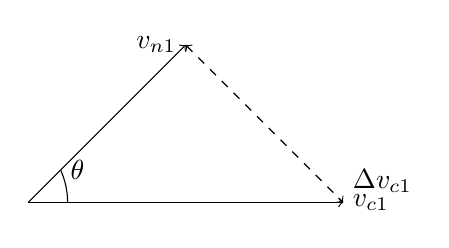
\begin{tikzpicture}
	
	\draw[->] (0, 0) -- (4, 0) node[anchor=west] {$v_{c1}$};
	\draw[->] (0, 0) -- (2, 2) node[anchor=east] {$v_{n1}$};
	\draw[<->, dashed] (2, 2) -- (4, 0) node[anchor=south west] {$\Delta v_{c1}$};
	\draw (0.5,0) arc (0:24:1) node[anchor=west] {$\theta$};
	
\end{tikzpicture}
\caption{A triangle showing a velocity $v_{c1}$ moving to another velocity $v_{n1}$. The amount of velocity to move $v_{c1}$ to $v_{n1}$ is called $\Delta v_{c1}$, which is effected by the angle $\theta$.}
\end{figure}

In order to make an inclination change, you have to exert a certain amount of thrust $\Delta v$ in order to create a path to a new orbit. The amount of $\Delta v$ required can be calculated using the cosine rule.
\begin{equation}
\Delta v^2 = (v_1^2 + v_2^2) - (2 v_1 v_2) \cos \theta
\end{equation}
\begin{center}
	In the case $v_1 = v_2 = v$
\end{center}
\begin{equation}
	\Delta v = 2v^2 (1 - \cos \theta)
\end{equation}

\newpage

\section{Escape Velocity}

\begin{figure}[h]
	\centering
	\begin{tikzpicture}
		% Grid for temporary reference

		% \draw[step=1.0cm,color=gray] (-5,-5) grid (5,5);
		% \filldraw[black] (0, 0) circle (2pt);

		% Lines and shapes
		\draw (1.5, 0) ellipse (1.5 and 1.5);
		\filldraw[black] (1.5,0) circle (2pt);	
		\draw (1.5, 0) -- (1.5, 1.5);
		\draw (1.5, 0) -- (1.5, -1.5);
		\draw (0, 0) -- (3, 0);
		\path[draw, ->, thick] (2.99, -0.1) --  (3, 0) node[anchor=north east] {$v_{c1}$};
		% Text, math stuff, and distance
		\draw (1.5, 0) -- (2.65, -1) node[anchor=north west] {$r_c$};
		\node[anchor=east] at (3.785, 0) {$r_1$};
		\node[anchor=west] at (-0.7, 0) {$r_2$};

		% path to new orbit
		\draw[dashed, thick] (0, 0) parabola[bend at end] (3, -6) node[anchor=north west] {$a = \infty$ or $r = \infty$};
	\end{tikzpicture}
	\label{fig: 4}
	\caption{When a certain amount of $\Delta v$ is applied to an orbit, the average (semi-minor) axis or the distance to the body being orbited is ``escaped''. Or, the influence from the body is removed to an extreme extent, and at all points, is influenced by a different body.}
\end{figure}
Recall Eq. (1.2), when we find a point where the semi-major axis is infinite

\begin{equation}
	v_{esc}^2 = \frac{2 \mu}{r} \,.
\end{equation}

However, when the distance is infinite,

\begin{equation}
	v_{\infty}^2 = -\frac{\mu}{a} \,.
\end{equation}

So, in order to get the escape velocity for both $a$ and $r$\footnote{It is worth noting to not do both equations simultaniously. Because if you treat both as infinity, they cancel out (or more specifically, can't add to eachother). However, if one is infinity, you can just take another out and derive to either $v_{esc}^2$ or $v_{\infty}^2$.}, 

\begin{equation}
	v_{cmbd}^2 = v_{esc}^2 + v_{\infty}^2 \,.
\end{equation}

\newpage

\section{Some general rocket design}

\subsection{Thrust-to-Weight-Ratio}

\begin{equation}
	\text{TWR } = \frac{F_T}{m g} > 1 \,,
\end{equation}

where

\begin{itemize}
	\item $F_T$: Thrust
	\item $m$: Mass
	\item $g$: Gravitational Acceleration (on earth, $g = 9.8 \frac{\text{m}^2}{\text{s}}$)
\end{itemize}

In plain english: Thrust must exceed the force of gravity.

\subsection{Combined Inspecific Impulse}

\begin{equation}
	I_{sp} = \sum_n \frac{F_n}{F_n / I_{sp n}} \,,
\end{equation}

where $n$ is the rocket. $n$ is more of an abstract way to represent a number of thrusters rather than writing down a bunch of terms. As-per-usual, 

\begin{itemize}
	\item $F_n$: Force of an $n$th rocket
	\item $I_{sp n}$: The inspecific impulse of an $n$th rocket
\end{itemize}

\subsection{Delta-v}

\begin{equation}
	\Delta v_{atm} = \ln \bigg( \frac{m_{\text{start}}}{m_{\text{end}}} \bigg) I_{sp} g \,.
\end{equation}

or when $g = 0$ in a vacumn

\begin{equation}
	\Delta v_{vac} = \ln \bigg( \frac{m_{\text{start}}}{m_{\text{end}}} \bigg) I_{sp} \,.
\end{equation}

In plain english: The amount of usable velocity in a rocket is a result of the mass of a rocket's full and empty mass, the specific impulse, and gravitational acceleration of a body (if a rocket is on, or flying in a planet).

\subsubsection{True Delta-v from $atm$ to $vac$}

\begin{equation}
	\Delta v_T = \frac{\Delta v_{atm} - \Delta v_{vac}}{\Delta v_{atm}} \times \Delta v_{vac} + \Delta v_{out}
\end{equation}

where $\Delta v_{out}$ is the amount of $\Delta v$ used to get out the atmosphere (or lack thereof).

We can view how starting $m_{start}$ is effected by a hypothetical $m_{end}$ and $I_sp$.\footnote{The maple worksheet should be in whatever git repository this is being hosted on.}

\begin{figure}[h]
	\centering
	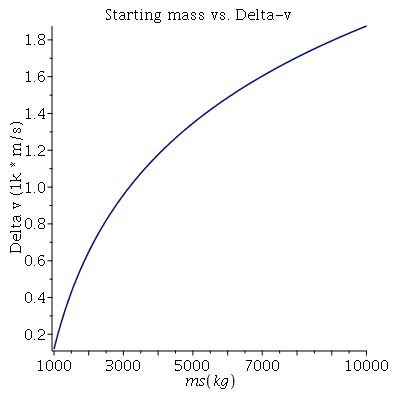
\includegraphics[scale=0.5]{ms_vs_delta-v}
	\label{fig: 5}
	\caption{In this case, I set $I_{sp} = 0.762244$ and $m_{end} = 854.15239$ in Maple.}
\end{figure}

\end{document}
